%	paper.tex	Toby Searle
%	Last modified: Fri 22 Jan 15:20:25 2016
%	using jfm template

\NeedsTeXFormat{LaTeX2e}

\documentclass{jfm}

\usepackage{graphicx}
\usepackage{natbib}
%%%%%%%%%%%Added to template:
\usepackage{caption,subcaption, mathtools} % add my own packages
\usepackage[section]{placeins}
\graphicspath{ {./images/} }
\newcommand\Wi{\mbox{\textit{Wi}}}
\newcommand{\dt}[1]{\frac{d #1}{d t}} %time deriv
\newcommand{\dy}[1]{\frac{\partial #1}{\partial y}}
%%%%%%%%%%%%%%%

% See if the author has AMS Euler fonts installed: If they have, attempt
% to use the 'upmath' package to provide upright math.
\ifCUPmtlplainloaded \else
  \checkfont{eurm10}
  \iffontfound
    \IfFileExists{upmath.sty}
      {\typeout{^^JFound AMS Euler Roman fonts on the system,
                   using the 'upmath' package.^^J}%
       \usepackage{upmath}}
      {\typeout{^^JFound AMS Euler Roman fonts on the system, but you
                   dont seem to have the}%
       \typeout{'upmath' package installed. JFM.cls can take advantage
                 of these fonts,^^Jif you use 'upmath' package.^^J}%
       \providecommand\upi{\pi}%
      }
  \else
    \providecommand\upi{\pi}%
  \fi
\fi

% See if the author has AMS symbol fonts installed: If they have, attempt
% to use the 'amssymb' package to provide the AMS symbol characters.

\ifCUPmtlplainloaded \else
  \checkfont{msam10}
  \iffontfound
    \IfFileExists{amssymb.sty}
      {\typeout{^^JFound AMS Symbol fonts on the system, using the
                'amssymb' package.^^J}%
       \usepackage{amssymb}%
       \let\le=\leqslant  \let\leq=\leqslant
       \let\ge=\geqslant  \let\geq=\geqslant
      }{}
  \fi
\fi

% See if the author has the AMS 'amsbsy' package installed: If they have,
% use it to provide better bold math support (with \boldsymbol).

\ifCUPmtlplainloaded \else
  \IfFileExists{amsbsy.sty}
    {\typeout{^^JFound the 'amsbsy' package on the system, using it.^^J}%
     \usepackage{amsbsy}}
    {\providecommand\boldsymbol[1]{\mbox{\boldmath $##1$}}}
\fi

%%% Example macros (some are not used in this sample file) %%%

% For units of measure
\newcommand\dynpercm{\nobreak\mbox{$\;$dyn\,cm$^{-1}$}}
\newcommand\cmpermin{\nobreak\mbox{$\;$cm\,min$^{-1}$}}

% Various bold symbols
\providecommand\bnabla{\boldsymbol{\nabla}}
\providecommand\bcdot{\boldsymbol{\cdot}}
\newcommand\biS{\boldsymbol{S}}
\newcommand\etb{\boldsymbol{\eta}}

% For multiletter symbols
\newcommand\Real{\mbox{Re}} % cf plain TeX's \Re and Reynolds number
\newcommand\Imag{\mbox{Im}} % cf plain TeX's \Im
\newcommand\Rey{\mbox{\textit{Re}}}  % Reynolds number
\newcommand\Pran{\mbox{\textit{Pr}}} % Prandtl number, cf TeX's \Pr product
\newcommand\Pen{\mbox{\textit{Pe}}}  % Peclet number
\newcommand\Ai{\mbox{Ai}}            % Airy function
\newcommand\Bi{\mbox{Bi}}            % Airy function

% For sans serif characters:
% The following macros are setup in JFM.cls for sans-serif fonts in text
% and math.  If you use these macros in your article, the required fonts
% will be substitued when you article is typeset by the typesetter.
%
% \textsfi, \mathsfi   : sans-serif slanted
% \textsfb, \mathsfb   : sans-serif bold
% \textsfbi, \mathsfbi : sans-serif bold slanted (doesnt exist in CM fonts)
%
% For san-serif roman use \textsf and \mathsf as normal.
%
\newcommand\ssC{\mathsf{C}}    % for sans serif C
\newcommand\sfsP{\mathsfi{P}}  % for sans serif sloping P
\newcommand\slsQ{\mathsfbi{Q}} % for sans serif bold-sloping Q

% Hat position
\newcommand\hatp{\skew3\hat{p}}      % p with hat
\newcommand\hatR{\skew3\hat{R}}      % R with hat
\newcommand\hatRR{\skew3\hat{\hatR}} % R with 2 hats
\newcommand\doubletildesigma{\skew2\tilde{\skew2\tilde{\Sigma}}}
%       italic Sigma with double tilde

% array strut to make delimiters come out right size both ends
\newsavebox{\astrutbox}
\sbox{\astrutbox}{\rule[-5pt]{0pt}{20pt}}
\newcommand{\astrut}{\usebox{\astrutbox}}

\newcommand\GaPQ{\ensuremath{G_a(P,Q)}}
\newcommand\GsPQ{\ensuremath{G_s(P,Q)}}
\newcommand\p{\ensuremath{\partial}}
\newcommand\tti{\ensuremath{\rightarrow\infty}}
\newcommand\kgd{\ensuremath{k\gamma d}}
\newcommand\shalf{\ensuremath{{\scriptstyle\frac{1}{2}}}}
\newcommand\sh{\ensuremath{^{\shalf}}}
\newcommand\smh{\ensuremath{^{-\shalf}}}
\newcommand\squart{\ensuremath{{\textstyle\frac{1}{4}}}}
\newcommand\thalf{\ensuremath{{\textstyle\frac{1}{2}}}}
\newcommand\Gat{\ensuremath{\widetilde{G_a}}}
\newcommand\ttz{\ensuremath{\rightarrow 0}}
\newcommand\ndq{\ensuremath{\frac{\mbox{$\partial$}}{\mbox{$\partial$} n_q}}}
\newcommand\sumjm{\ensuremath{\sum_{j=1}^{M}}}
\newcommand\pvi{\ensuremath{\int_0^{\infty}%
  \mskip \ifCUPmtlplainloaded -30mu\else -33mu\fi -\quad}}

\newcommand\etal{\mbox{\textit{et al.}}}
\newcommand\etc{etc.\ }
\newcommand\eg{e.g.\ }


\newtheorem{lemma}{Lemma}
\newtheorem{corollary}{Corollary}

\title[Viscoelastic Kelvin-Helmholtz instabilty]{Viscoelastic Kelvin-Helmholtz instability}

\author[T. W. Searle and A. N. Morozov]%
{T. W. Searle$^1$ and A. N. Morozov$^1$%
  \thanks{Email address for correspondence: jfm@damtp.cam.ac.uk},\ns
}

% NOTE: A full address must be provided: department, university/institution, town/city, zipcode/postcode, country.
\affiliation{$^1$SUPA, School of Physics and Astronomy, University of Edinburgh, Mayfield Road,
Edinburgh, EH9 3JZ, UK\\[\affilskip]
}

\pubyear{2013}
\volume{650}
\pagerange{119--126}
% Do not enter received and revised dates. These will be entered by the editorial office.
\date{?; revised ?; accepted ?. - To be entered by editorial office}
%\setcounter{page}{1}
\begin{document}

\maketitle

\begin{abstract}
  Abstract goes here. Abstract goes here. Viscoelastic Kelvin-Helmholtz instability. 
\end{abstract}

\begin{keywords}
Authors should not enter keywords on the manuscript, as these must be chosen by
the author during the online submission process and will then be added during
the typesetting process (see
http://journals.cambridge.org/data/\linebreak[3]relatedlink/jfm-\linebreak[3]keywords.pdf
for the full list)
\end{keywords}

\section{Introduction}

It was long thought that the elasticity of a viscoelastic fluid only served to
dampen instability. This view stems from early results showing that drag in a
turbulent Newtonian flow can be reduced by the addition of small amounts of
viscoelastic fluid \citep{Toms1977}. Although drag reduction has been studied
for a long time, studies on turbulence without inertia \citep{Larson1990,
Groisman2000} give reason to believe that there are purely elastic bulk
instabilities present in elastic fluids relevant to industry.  This purely
elastic turbulence is present at very low Reynolds number, where it is driven
by the elasticity of a polymeric flow rather than its inertia. 

\subsection{Exact coherent structures and Turbulence}

In 1997 Fabian Waleffe identified a Newtonian self sustaining process in plane
Couette flow \citep{Waleffe1997}. Streamwise rolls redistribute the streamwise
velocity into a streaky flow. This streaky flow is unstable through a
Kelvin-Helmholtz instability leading to a symmetry bifurcation to a three
dimensional flow. Finally, the nonlinear effects due to this instability
re-energises the original streamwise rolls. This exact solution to the
Navier-Stokes equations is thought to be a component of the transition to
turbulence. In 1998 Waleffe constructed a bifurcation diagram for this exact
solution \citep{Waleffe1998} containing what looks like a bifurcation from
infinity, just the behaviour expected of the transition to turbulence in plane
Couette flow.

Using this work in Newtonian fluid dynamics as a template for the structure of
purely elastic turbulence reveals a similar pattern of streaks and, a similar
self-sustaining process \citep{Searle2016a}. An important step towards
explaining this process in purely elastic flows is establishing the mechanism
by which the streaks become unstable. It seems this is also a Kelvin-Helmholtz
instability as the streaks shear with the rest of the fluid.  The
Kelvin-Helmholtz instability is integral to the transition to turbulence in
Newtonian fluids. It is hoped that by finding a purely elastic version of this
instability, we might be able to probe one of the important mechanisms for the
transition to purely elastic turbulence, One that is presumably present in
other contexts, such as the oscillatory channel flow problem of
\cite{Searle2016b}. To explore this mechanism in the purely elastic regime we
have constructed a simple model system of a shearing viscoelastic fluid.

\subsection{Shear flow instabilities of Non-Newtonian fluids}

The shear flow instability we are interested in relates to many other
instabilities in both Newtonian and Non-Newtonian fluids where the fluid
inertia is not dominant. These instabilities mostly relate to a flow of two
fluids with differing properties and an instability at the interface between
them. I will break them up into 4 classes, Newtonian viscously stratified, shear
thinning viscously stratified, Shear banded and Elastically stratified
instabilities.

\subsection{Viscous two layer Newtonian shear flows}

In 1967 Yih \citep{Yih1967} performed a long wavelength analytic stability
calculation of two Newtonian fluids in two-layer viscously stratified plane
Couette and plane Poiseuille flows. This instability was shown to be an
instability of the interface. Many subsequent authors copy Yih's technique and
notation.

In 1983 the viscous stratification instability was studied in a flow which is a
close relation to ours. Hooper and Boyd tackle the Newtonian two-layer viscous
instability \citep{Hooper1983} in a flow of two fluids both in unbounded
Couette flow with a jump in the shear rate at the interface. They use both
numerical and shortwave asymptotic techniques to obtain that the shortwave
instability is always unstable without surface tension. Hinch \citep{Hinch1984}
explained the mechanism of the Hooper and Boyd viscous stratification of above.
Says that this instability ought to be unimportant since it will be damped by
surface tension.

Renardy \citep{Renardy1985} repeats both the Yih and the Hooper Newtonian fluid
problems but does a full numerical linear stability analysis using a
Chebyshev-Tau method of Orszag. The problems with and without walls yield
approximately the same critical Reynold's number. Above this the unstable
eigenmodes for each problem are approximately the same. They include surface
tension, density, viscosity, and volume fraction ratio.  \citet{Hooper1985}
then looked at a thin film on top of another Newtonian fluid via a long
wavelength linear stability analysis. Suggest a mechanism based on the lag
between phases of velocity and phase of interface.  \citet{Hooper1985} then
looked at the nonlinear stability of stratified Couette-Poiseuille flow. They
performed a weakly nonlinear analysis to transform the problem to a
Kuramoto-Sivishinsky equation and they don't find any travelling waves. Renardy
\citep{Renardy1989} also looked at this nonlinear stability problem and found
small amplitude travelling waves.  \citet{Yiantsios1988} do a numerical linear
stability of two superposed Newtonian fluids, looking at the short wave
asymptotics like Hooper and Boyd but include surface tension and gravitational
effects.

\subsection{Viscous two layer shear thinning Non-Newtonian shear flows}

Waters \citep{Waters1983} does a long wavelength linear stability analysis for
shear thinning power law fluids in plane Couette flow and claims that shear
thinning has a large effect. Wong and Jeng \citep{Wong1987} do a long wave
linear stability analysis for co-extruded pipe flow of Ellis model shear
thinning non-Newtonian fluids. Find that if inner/outer fluid is more viscous
shear thinning will stabilize/destabilize the flow.

Weinstein \citep{Weinstein1990} examined the flow of shear thinning fluids down
and incline. Use the Carreau model and look at multilayered flow using analytic
asymptotics as well as a finite difference shooting method for the eigenvalues.
Find that effects of shear-thinning are complicated.

Pinarbasi \citep{Pinarbasi1995} in 1995 looked at two shear thinning models for
the 2-layer Poiseuille flow, Carreau-Yasuda and the Bingham like model. They
use a pseudospectral method eigensolver to show that shear thinning
destabilizes. 

\subsection{shear banded Non-Newtonian shear flows}

McLeish \citep{McLeish1987} look at the stability of the interface between two
phases of linear polymer melts using the Doi-Edwards model. Show that a
shear-banded state has an unstable interface between the fluids. Claims that
the normal stress effect determines instability. Renardy \citep{Renardy1995a}
returned to this problem to examine how a shear banding instability might be
responsible for spurt in two layer Couette flow.  Used the Johnson-Segalman
model with a pseudospectral eigenvalue solver. 

Mike Graham does a review of the sharkskin instability in \citep{Graham1999}
which discusses a lot of previous work and which I found interesting as an
insight into how the wall-slip and shear-banding instability factions think
about melt fracture.

Fielding \citep{Fielding2005} looks at the linear stability of the shear-banded
flow problem. Use the Johnson-Segalman model, finds that the shear banded state
can be linearly unstable. The mechanism is not clear. Then Wilson
\citep{Wilson2006} has a nice little article discussing how an instability can
depend or not on changing the constitutive model. Using a small amount of
diffusion in the diffusive Johnson-Segalman model doesn't effect the
instability even though the limit of zero diffusion is singular.

Fielding and Wilson \citep{Fielding2010} look at the shear banding interfacial
instability in plane Poiseuille flow via the diffusive Johnson Segalman model.
They do both a numerical linear stability and find nonlinear travelling
waves.

\citet{Nicolas2012} look at the shear banding instability, this
time in Taylor-Couette flow via the diffusive Johnson-Segalman model. Find a
previously unnoticed azimuthally wavy bulk instability. I particularly enjoyed
the comparison with the co-rotating problem where there is no shear band.

\subsection{Elastic multilayer Non-Newtonian shear flows}

The study of an elastically stratified shear flow began in 1969 when Li
\citep{Li1969} examined two Oldroyd-B fluids with different viscosities and
elasticities. This was a asymptotic expansion of the linear stability to long
wave length disturbances along the same lines as \citet{Yih1967}. They found
that elasticity can both stabilize and destabilise the flow. This study along
with some subsequent ones \citep{Waters1987, Anturkar1990}, used an incorrect
boundary condition for the traction at the interface between the fluids. Chen
\citep{Chen1991b} later corrects this mistake, and subsequent studies including
all the papers by Renardy contain the correct boundary condition.

\citet{Khan1976} studied an experimental realisation of the plane Poiseuille
flow of two viscoelastic fluids in a duct. They find that the influence of
viscosity dominates over that of elasticity stratification in their flow. They
attempt some analytic and numerical work on the Coleman-Noll second order fluid
to back up their experiments, but they use the wrong interface traction
boundary condition and their methods look dodgy. In \citet{Khan1977} the same
authors publish a flawed theory paper using the same constitutive model.

\citet{Han1985} perform a co-extrusion experiment on a pipe flow of two polymer
melts. Mainly this is just cross-sections of the extrudate showing that lower
viscosity component wraps higher viscosity component. They have no
birefringence data but somehow they do get some normal stress data. They claim
that the viscous stratification is more important than the elastic for their
system.

Waters and Keeley \citep{Waters1987} use an Newtonian fluid and power-law shear
thinning Oldroyd-B fluid in stratified plane Couette flow. They do long wave
asymptotics. Again, this paper uses the incorrect traction boundary condition
at the interface.  Renardy \citep{Renardy1988} looked at the stability of the
interface of two layer Couette flow of UCM fluids via short wave asymptotics
and a Chebyshev-tau method. They find elastic differences between the layers
alone can stabilize or destabilize the flow. Claim that elasticity can enhance
the lubrication effect. 

Anturkar \citep{Anturkar1990} do a problem involving multiple viscoelastic
layers in planar co-extrusion. Do numerical and analytical linear stability
analysis on the Oldroyd-B + Carreau shear thinning model.  Again they use the
incorrect traction boundary condition at the interfaces between the fluids.

Chen \citep{Chen1991a} looked at the elastic instability in the co-extrusion of
UCM fluids in a pipe flow. He performed a long wavelength linear stability
analysis and found an elastic instability. In \citep{Chen1991b} he then went on
to look at the Couette flow of viscoelastic fluids and corrects the error in
previous papers \citep{Li1969, Waters1987, Anturkar1990} for the interface
traction boundary condition. Previous authors took the boundary condition on
the unperturbed interface between the fluids, rather than the perturbed one.
It is demonstrated that you can get a purely elastic linear instability via a
long wave asymptotic analysis. The linear stability of a two layer film of UCM
fluids down an inclined plane was examined by a long wave asymptotic analysis
as well as using a pseudospectral method \citep{Chen1992a}. The result is that
there is an instability when the more elastic component is next to the wall.
The shortwave instability of the pipe co-extrusion flow is examined in
\citep{Chen1992b} using the UCM model. Hypothesis formed about the origin of
sharkskin being due to differing elastic properties of the fluid close to the
wall.  Find growth rates are in fact higher for the elastic instabilities than
the viscous Newtonian ones in some settings. Many of the previous viscoelastic
references are mentioned in \citep{Larson1992}.

\citet{Su1992a} find a purely elastic interfacial instability in superposed
Poiseuille flow of Oldroyd-B fluids. This is a Plane Poiseuille flow version of
\citep{Chen1992a}. Long wave asymptotic and some numerical linear stability
using a pseudospectral technique. Show that strength of elastic instability is
comparable to that of the Newtonian viscous one. They have some low $\beta$ low
$\Rey$ results. In \citet{Su1992b} they look at converging and parallel channel
co-extrusion of two truncated power law Oldroyd-B fluids.  Find that shear
thinning has a bigger effect than elasticity.  Many phase diagrams.

Hinch, Harris and Rallison \citep{Hinch1992} provide a general understanding of
the mechanism behind Chens pipe elastic stratification instability
\citep{Chen1991a}. They look for an arbitrary constitutive model and include
the effects of jumps in the first and second normal stress differences in order
to expose how the traction boundary condition can bring about instability.

Wilson and Khomami \citep{Wilson1992, Wilson1993a, Wilson1993b} performed a
three part experimental investigation of the interfacial instabilities in
multilayered flow of viscoelastic liquids. They can generate disturbances of
particular wavelengths in their setup, to probe the dispersion relation. The
compare with the Oldroyd-B with power law shear thinning fluid and find
reasonable agreement. They also examine nonlinear effects \citep{Wilson1993a}
using the same apparatus and they find that there are shear stress imbalances
in their flows supporting the proposed instability mechanism, and they show
that differences in the normal stress difference enough to change the
dispersion relation, lending support to the presence of an elastic instability.
Find a supercritical bifurcation and it looks like the interface rolls up in a
Kelvin-Helmholtz like way. They say they see things similar to predictions made
in \citet{Renardy1989}. No subcritical bifurcation is observed. Complex 3D
pattern occurs which made it difficult to look at the purely elastic effects
divorced from the viscous stratification effects. For compatible polymers
\citep{Wilson1993b} they observe suppression of the growth rate due to diffusive
and convective mixing.

Chen \citep{Chen1993} looked at the stability of the interface in the pipe
co-extrusion experiment via pseudospectral eigenvalue solver using the
Oldroyd-B model. Discusses two kinds of interfacial instability, capillary
instability due to surface tension and elastic due to first normal stress
difference.  Explains again the Hinch mechanism, but perhaps easier to
understand. The Capillary instability can be stabilised by the elasticity
stratification. In 1994 \citep{Chen1994} Chen examines the instability of a
large $\Rey$ flow of a Newtonian fluid over an Oldroyd-B fluid. There is an
asymptotic expansion for the linear stability in the short wave limit.

\citet{Azaiez1994} do the linear stability of a free shear flow of the
Oldroyd-B, co-rotational Jefferys and Gisekus fluids. Find suppression of the
Newtonian Kelvin-Helmholtz instability. They do asymptotic long wave linear
stability such that the Reynold's number is small but finite and the
Weissenberg number is large with a constant elasticity. They also do a
numerical linear stability via an orthogonal shooting algorithm. In the
appendix of this paper Hinch \citep{Azaiez1994} takes the long wavelength limit
of their problem in a far more elegant way and exposes a stabilisation
mechanism based on elastic hoop stresses in the curved streamlines.

Renardy returned to the two-layer flow of the elastically stratified UCM model
to look at the weakly nonlinear problem \citep{Renardy1995b}. They redid the
numerical linear stability analysis and then found the bifurcations were
supercritical. Coward and Renardy \citep{Coward1997} looked at a thin film
core-annular pipe flow of UCM fluids via a weakly nonlinear analysis.

Wilson and Rallison \citep{Wilson1997} looked at the short wave instability of
the elastically stratified two layer plane Poiseuille flow of Oldroyd-B liquids.
This was an asymptotic linear stability analysis for short waves. Possibly this
is a different mechanism than the Hinch one because it happens for short
wavelengths. 

In 1997, Laure \citep{Laure1997} looked at the linear stability of a multilayer
plane Poiseuille flow of Oldroyd-B fluids. They did a long wave asymptotic
analysis in the $\Rey \rightarrow 0, \Wi \neq 0$ limit. They also did some
numerical calculations. They assume that viscous and elastic effects are
additive in the dispersion relation. \citet{Ganpule1998} thinks this is wrong.
In the \citet{Ganpule1998} paper they also look at four models, UCM, multimode
Gisekus, Gisekus and modified PTT. They repeat the linear stability analysis
and do a perturbation energy analysis using the UCM model. They also compare
all their results to experiments in \citep{Khomami1997}. Those experiments are
performed on the multilayer pressure driven flow of polymeric melts. In
\citet{Ganpule1999} they published a similar theory paper but on just two
layers in more detail rather than a multilayered flow. Show how the Oldroyd-B
is qualitative match to experiments but gets the wrong growth rates. Attribute
this to shear thinning of the experiment in \citep{Khomami1997}. Again they use
an energy disturbance analysis to study the mechanism and it seems they agree
with the Hinch mechanism of \citep{Hinch1992}.  It seems whatever the mechanism
they settle on in this paper, Miller and Rallison disagree with it in
\citep{Miller2007a}. 

\citet{Scotto1999} looks at the linear stability of a three layer Poiseuille
flow of Oldroyd-B fluids using a Chebyshev-tau method. I think they do the
dodgy thing of adding together affects from the viscous and elastic terms in
the dispersion relation.

Renardy \citep{Renardy1999} looks at the spanwise instability between two
Gisekus Couette layers with only a second normal stress jump. They use a fully
spectral Chebyshev-Tau method and find that short waves are always unstable and
without surface tension whereas long waves depend on the depth ratio.

\citet{Wilson1999a} looked at the instability of channel flows of
elastic liquids having continuously stratified polymer concentration and $\Wi$.
They look at the long wavelength limit of the Oldroyd-B model using what I
think is a similar method to to Hinch in \citet{Azaiez1994}. Then they do
linear stability using a shooting Newton-Rhaphson method. They compare the
results of the Oldroyd-B model to a White-Mieztner fluid. Conclude that
blurring of the interface between elasticities would suppress the instability,
so it is not likely to be responsible for sharkskin. Their instability looks to
be the closest to ours as far as I can gather.

\citet{Wilson1999b} concerns the structure of the eigenvalue spectrum
for the instability of UCM and Oldroyd-B fluids in the two-layer channel flow
problem. Possibly a useful comparison there for our eigenvalue spectra.

Khomami et al performed linear stability analysis of a two layer Oldroyd-B and
Newtonian pressure-driven channel flow and compared it to an experiment with an
elastic Boger fluid and a Newtonian fluid in \citep{Khomami2000a, Khomami2000b}.
They found that they could fit their experiments with the Oldroyd-B model and
find that their experiments saturated to 2D structures unlike the 3D structures
seen in \citep{Khomami1997} and they suggest that it is because this was a
second normal stress effect a la \citep{Renardy1999} which is not present in the
current experimental setup. Their second paper, \citep{Khomami2000b} does the
theoretical weakly nonlinear stability analysis and finds supercritical
bifurcations as expected.

For some entertainment if you have read this far, \citep{Renardy2000} is a
review article which I think states that my PhD is pointless, "Much early work
on stability of shear flows was motivated by the desire to explain melt
fracture (‘viscoelastic turbulence’) as a result of an instability similar to
the laminar/turbulent transition in Newtonian flows. This is no longer believed
to be a realistic proposition."

Brady \citep{Brady2002} claim to have a generic instability that explains
Renardy's \citep{Renardy1999} second normal stress jump result, look at a
variety of flows including falling film and Newtonian fluid of non-Newtonian
flow. They use their own viscous-suspension flow constitutive model and
examine the effects of a jump in the second normal stress.

Meulenbroek \citep{Meulenbroek2004} show that there is weakly nonlinear
subcritical instability in Poiseuille flow of Oldroyd-B fluids. But seeing as
you are an author I expect you know that better than me.

Miller  looks at the interfacial instability between sheared UCM and Oldroyd-B
liquids in channel flow \citep{Miller2007a} and a pipe flow
\citep{Miller2007b}. They don't like the distinction between short and long
wave instabilities. They don't think that surface tension stabilises as claimed
in \citep{Chen1992b}. Look at a new limit, where $L < k^{-1} < U_{0} \lambda$
the wavelength is long compared to the channel width but short compared to the
relaxation length scale. They use a combination of short and long wave
techniques. They claim that their instability has a different origin to the
Hinch one I think.

Bonhomme, O, Morozov \citep{Bonhomme2011} find an elastic instability in the
core annular flow of two different Oldroyd-B fluids and perform short wave
linear stability asymptotics. Also some experiments, but I imagine you would
know all about this.

Wongsomnuk, \citep{Wongsomnuk2000} do a little experiment to show the sharkskin
instability onset. I am sure there is probably a better experiment for this out
there, but this is just the one that came up.

\citet{Yoo2013} does something that may be related to our instability, but
it is a long shot. They look at the effect of viscoelasticity on an instability
at the interface between lamellar phases with different orientations under
oscillatory shear.  They use a linear constitutive law which I don't recognise.

\citet{Dubief2013} looks at the mechanism of elasto-inertial
turbulence in \citet{Samanta2013}. Possibly related to our instability,
but we have talked about this instability before and I don't think Yves has
convinced you it exists yet?

Mahdaoui \citep{Mahdaoui2013} do a numerical investigation of the co-extrusion
instability. They use a complicated multiscale simulation technique on the
Carreau-Yasuda multimode Johnson-Segalman model in 2D along with some possibly
molecular dynamics techniques in areas which are hard to resolve.

Beaumont \citep{Beaumont2013} do some experiments looking at turbulent flows in
a Taylor-Couette flow of purely elastic wormlike micelles. Find inhomogeneous
turbulence and suggest the existence of a bulk instability.

Fardin \citep{Fardin2014} has a review article on the Taylor-Couette flow for
soft matter. It references you a lot and discusses the possibility of a purely
elastic KH instability. No doubt you are partially responsible for getting that
line put in there!

McKinley \citep{McKinley1996} gives us the geometrical $\Wi$ scaling. Zilz 2012
\citep{Zilz2012} have nice serpentine channel purely elastic flow which
supports the Pakdel-McKinley condition if we choose to use it.

\section{Problem formulation}

We present a linear stability analysis of the Kelvin-Helmholtz instability in
the purely elastic regime using direct numerical simulation of both the
Oldroyd-B and FENE-P constitutive models for a polymeric fluid. The purely
elastic fluid is found to be unstable at sufficiently high Weissenberg number,
the key dimensionless number for turbulence without inertia in viscoelastic
flows. This is the ratio of the normal stress to the shear stress of the
polymeric component of the fluid $Wi = \frac{N_{1}}{\sigma} = \lambda
\dot{\gamma}$ where $\dot{\gamma}$ is the shear rate.  The growth rate of the
largest growing eigenmode of the instability is found to increase with
increasing Weissenberg number for low Reynold's number. This behaviour is
consistent across both the Oldroyd-B and FENE-P models.

The system we use for our analysis uses a hyperbolic tangent shaped laminar
profile for the streamwise velocity across a channel, where the instability
takes place between $y = \pm \Delta$. $y=0$ is the centreline of the channel,
so that if $\Delta << 1$ the flow can be said to be a free shear instability.
This gives a base flow profile, 
\begin{align} 
    U(y) &= \tanh \left( y/\Delta
    \right) \coth \left( 1/\Delta \right) \nonumber\\ V &= 0 \nonumber \\
    T_{xx}(y) &= 2 Wi \left( \dy{U} \right)^{2} \nonumber \\ T_{xy}(y) &=
    \dy{U} \nonumber \\ T_{yy}(y) &= 0 \nonumber \label{eq:KH_laminar_profile}
\end{align}
$U$ and $V$ are the base streamwise (x) and wall normal (y) velocities
respectively. $T$ is the base stress tensor. We use Gauss-Labatto points in the
wall-normal ($y$) direction for the base profile, and decomposed the
disturbances to this flow into Fourier modes.  
\begin{equation} 
    g(y) = \sum\limits_{n=-N}^{N} \widetilde{g}(y) e^{ikx + \lambda t} 
\end{equation}
for all disturbance variables $g = u, v, p, \tau_{i,j}$. Where $N$ is the
number of Fourier modes, $k$ is the streamwise wavenumber of the disturbance
and $\lambda$ is the growth rate of the mode. This program uses two domains of
pseudo-spectral points to give increased resolution in the centre of the
simulation. The simulation was also repeated using a code for which the system
of points was stretched using: 
\begin{align} 
    z_{u} &= \frac{y_{u}}{1-y_{u}} \\
    z_{b} &= \frac{y_{b}}{1+y_{b}} \\ U     &= \tanh{z/\Delta}
    \label{eq:KH_inf_profile} 
\end{align} 
This system ought to be completely insensitive to the boundary conditions at
the walls so we refer to it as 'free shear' throughout this manuscript. 

The dimensionless quantities used throughout are non-dimensionalised relative
to the instability size, $\Delta$, rather than the total simulation size. The
obvious reason for this is that $\Delta$ is the length scale for the free shear
instability.

In order to simulate this flow, we used an Oldroyd-B fluid with very low
Reynolds number $\Rey \leq 0.01$ and a small ratio between the solvent and total
viscosities $\beta = \frac{\mu_{s}}{\mu_{s}+\mu_{p}}$. This approximates a
purely elastic fluid, where the polymer contribution to the stress on the fluid
is much larger  than the solvent contribution. The Oldroyd-B Navier stokes and
constitutive equations are then: 
\begin{align} 
    Re \left[ \dt{\mathbf{v}} +
    \mathbf{v} \cdot \nabla  \mathbf{v} \right] &= - \nabla p + \beta
    \nabla^{2} \mathbf{v} + \frac{1-\beta}{Wi} \nabla \cdot \mathbf{\tau} \\
    \dot{\tau}/Wi + \overset{\nabla}\tau &= \left(\nabla \mathbf{v}\right)^{T}
    + \nabla{\mathbf{v}} 
\end{align} 
With $\mathbf{v}$ as the total (base flow and disturbance) velocity and $\tau$
as the total stress in the polymeric fluid. The FENE-P viscoelastic fluid has
the advantage of being similarly easy to simulate, but also including a finite
extensibility for the polymers. This leads to a stress which depends on a
conformation tensor ($\mathbf{C}$) for the polymer dumbbells via a non-linear
spring force:

\begin{equation} \mathbf{\tau} = \frac{1-\frac{3}{L^{2}}}{1 +
	\frac{L^{2}}{tr(\mathbf{C^{2}})}} \end {equation}

\begin{figure} 
    \centering 
    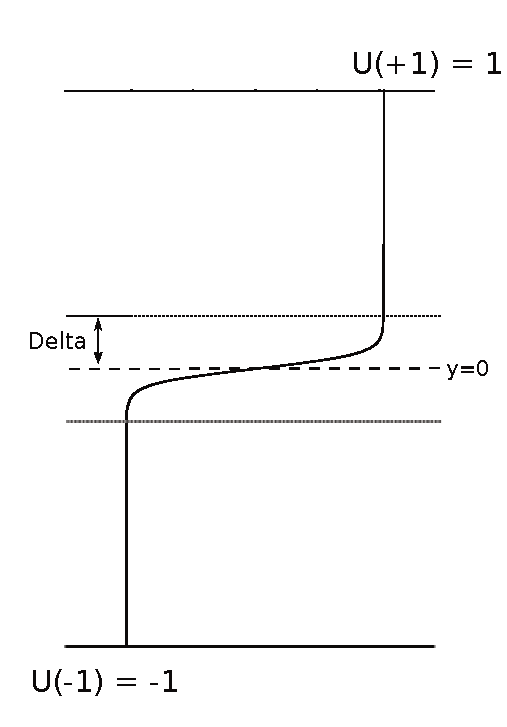
\includegraphics[width=0.3\textwidth]{KH_diagram}
    \caption{diagram of the system} 
    \label{fig:diagram} 
\end{figure}

Again, we used Gauss-Labatto points in the wall normal direction and Fourier
modes in the streamwise direction.

\section{A purely elastic instability}

At low Reynolds number, low $\beta$ and sufficiently large Weissenberg number
we observe an instability across a range of streamwise disturbance wavenumbers.
This leads us to suppose that this instability might be a plausible cause for a
self-sustaining process in viscoelastic plane Couette flow, similar to that
observed by Waleffe.

The instability remains unchanged under variation of $\Delta$ at low $\Delta$,
proving that it is a free shear instability. Although the instability appears
to require some inertia in the fluid, it is still present for  $\Rey = 0.01$,
far lower than the usual threshold of $\Rey = 1000$ for a Newtonian
Kelvin-Helmholtz instability.

We see an instability grow from around $k \sim 0.06$ and move to lower $k$ as
the Weissenberg number increases (figure \ref{fig:dispersions_low_Re}). The
height of the instability also increases with increasing Weissenberg number
(figure \ref{fig:inf_low_Re}). 

\begin{figure} 
    \centering 
    \begin{subfigure}[b]{0.48\textwidth} 
	\centering
	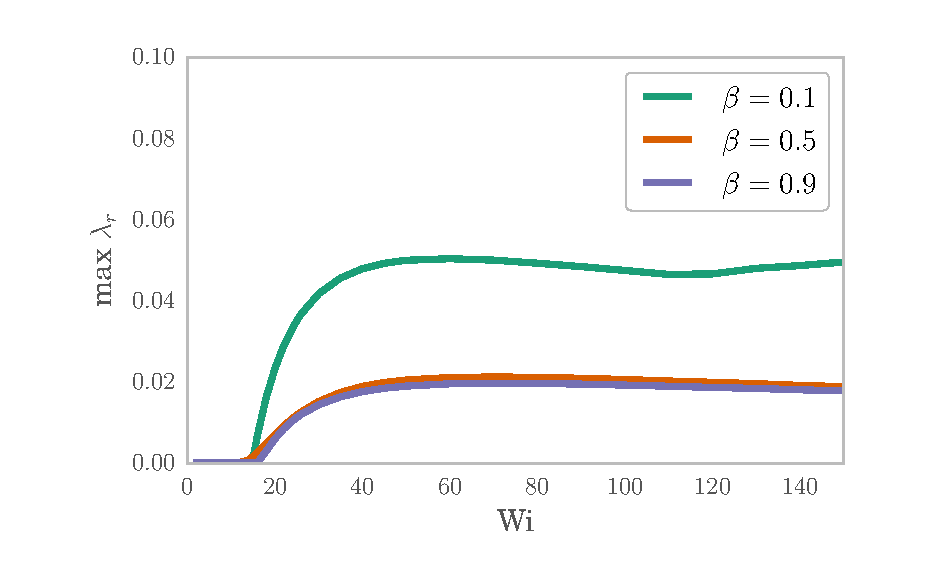
\includegraphics[width=\textwidth]{inf_purely_elastic} 
	\caption{}
	\label{fig:inf_low_Re} 
    \end{subfigure} ~
    \begin{subfigure}[b]{0.48\textwidth} 
	\centering
	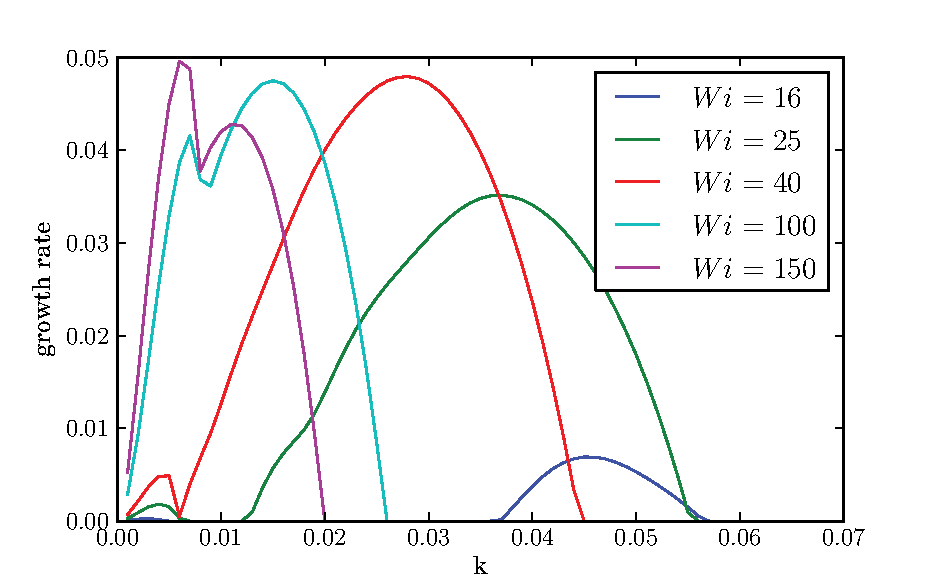
\includegraphics[width=\textwidth]{inf_dispersions_low_Re} 
	\caption{}
	\label{fig:dispersions_low_Re} 
    \end{subfigure} 
    \caption{
	a) Free shear version of the instability. Plot of the maximum growth
	rate against Weissenberg number at $\Rey = 0.01$. b) Dispersion
	relations at various Weissenberg numbers to accompany the trend in
	figure a).
    } 
\end{figure}

The dispersion relation saturates at $Wi \sim 50$ and remains approximately
constant with increasing Weissenberg number. The dispersion relation for the
instability remains broad in $k$ until $Wi \sim 100$ where a new eigenvector
becomes dominant.

\begin{figure} 
    \centering 
    \begin{subfigure}[b]{0.48\textwidth} 
	\centering
	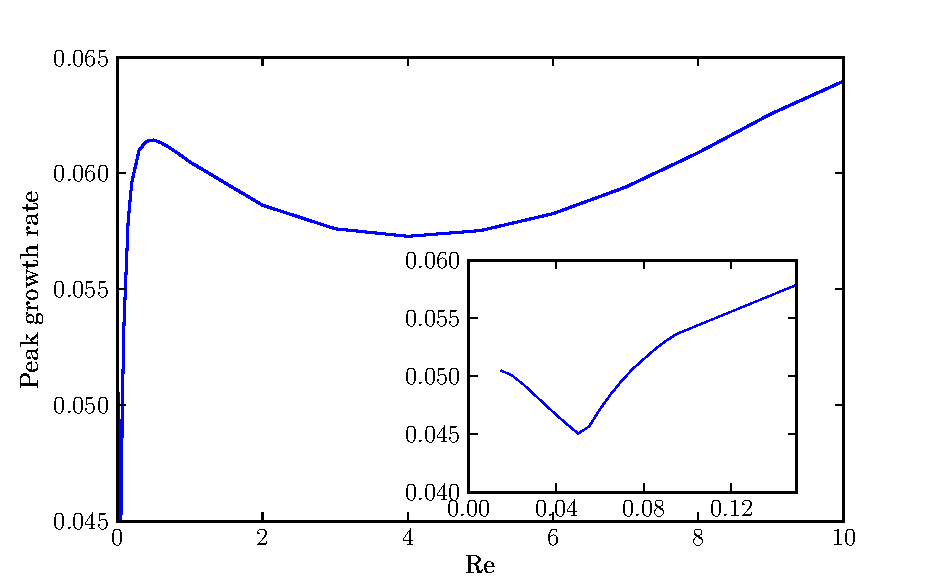
\includegraphics[width=\textwidth]{inf_vary_Re} 
	\caption{}
	\label{fig:inf_vary_Re} 
    \end{subfigure} ~
    \begin{subfigure}[b]{0.48\textwidth} 
	\centering
	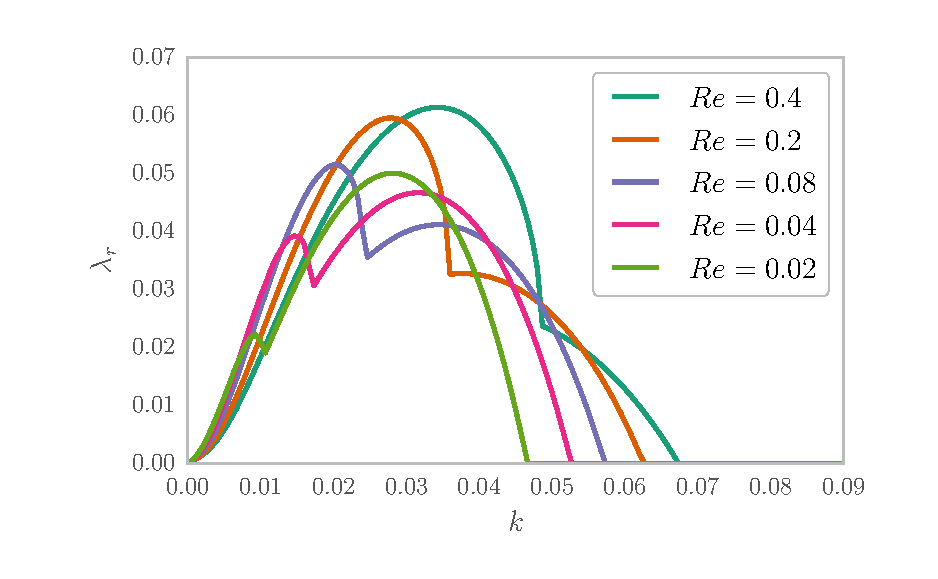
\includegraphics[width=\textwidth]{inf_dispersions_low_Wi} 
	\caption{}
	\label{fig:dispersions_low_Wi} 
    \end{subfigure} 
    \caption{ 
	a) Free shear version of the instability. Plot of the maximum growth
	rate against Reynold's number with $\Wi=50$. b) Dispersion relations at
	various Reynold's numbers to accompany the trend in figure a).  
    }
\end{figure}

As the Reynold's number is reduced, new eigenvalues become dominant. Although
the dominant eigenvalue changes the flow is still unstable, even down to $\Rey
= 0.01$ (see figures \ref{fig:inf_vary_Re} and \ref{fig:dispersions_low_Wi}).


\subsection{ Shear instability with walls}

If we examine the eigenvectors of the instability, we see that there are very
large polymer stresses in the $\pm \Delta$ region. This corresponds to the
large shear rate brought about as the two flows pass each other. Examining the
flow field, we see that there are large vortices arranged with opposite
rotational directions above and below the shear region which extend almost to
the walls. 

\begin{figure} \begin{subfigure}[b]{\textwidth} 
	\centering
	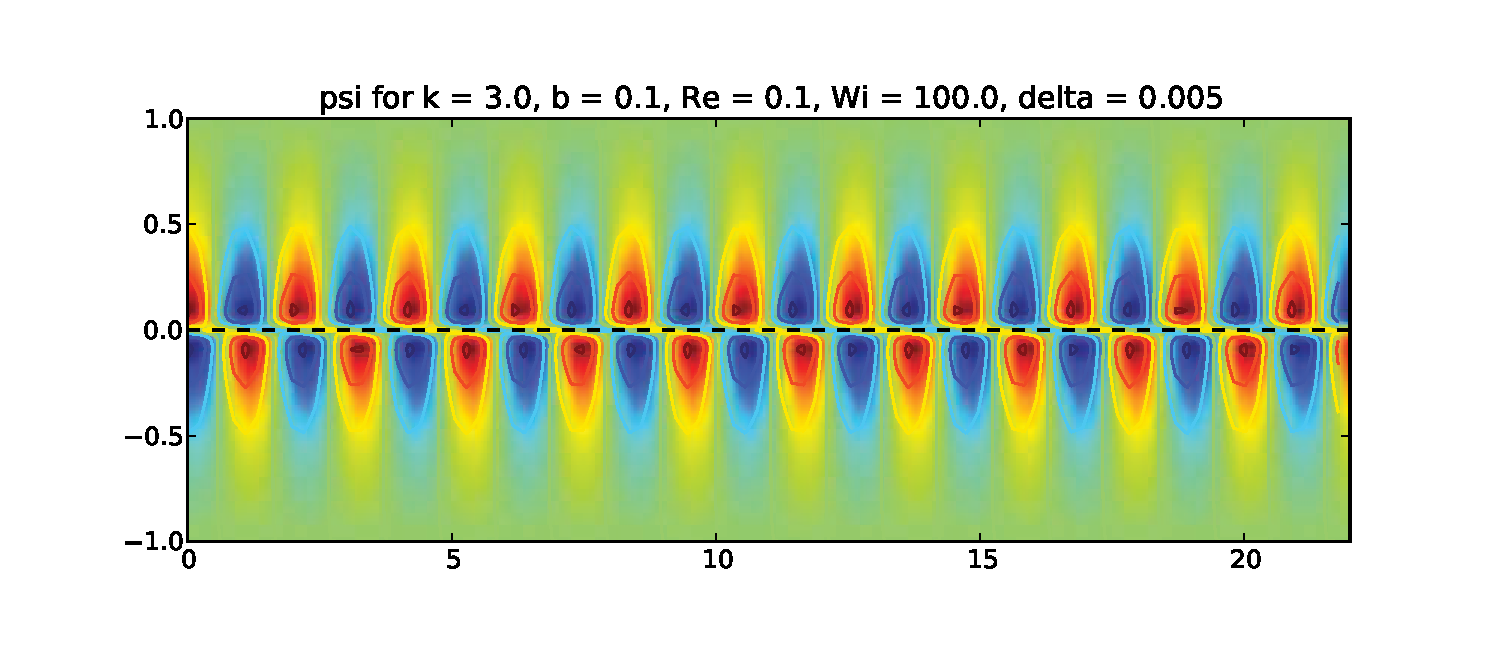
\includegraphics[width=\textwidth]{psi_low_delta}
	\caption{}
	\label{fig:psi_low_delta}
    \end{subfigure} \vspace{1 mm}
    \begin{subfigure}[b]{\textwidth}
	\centering
	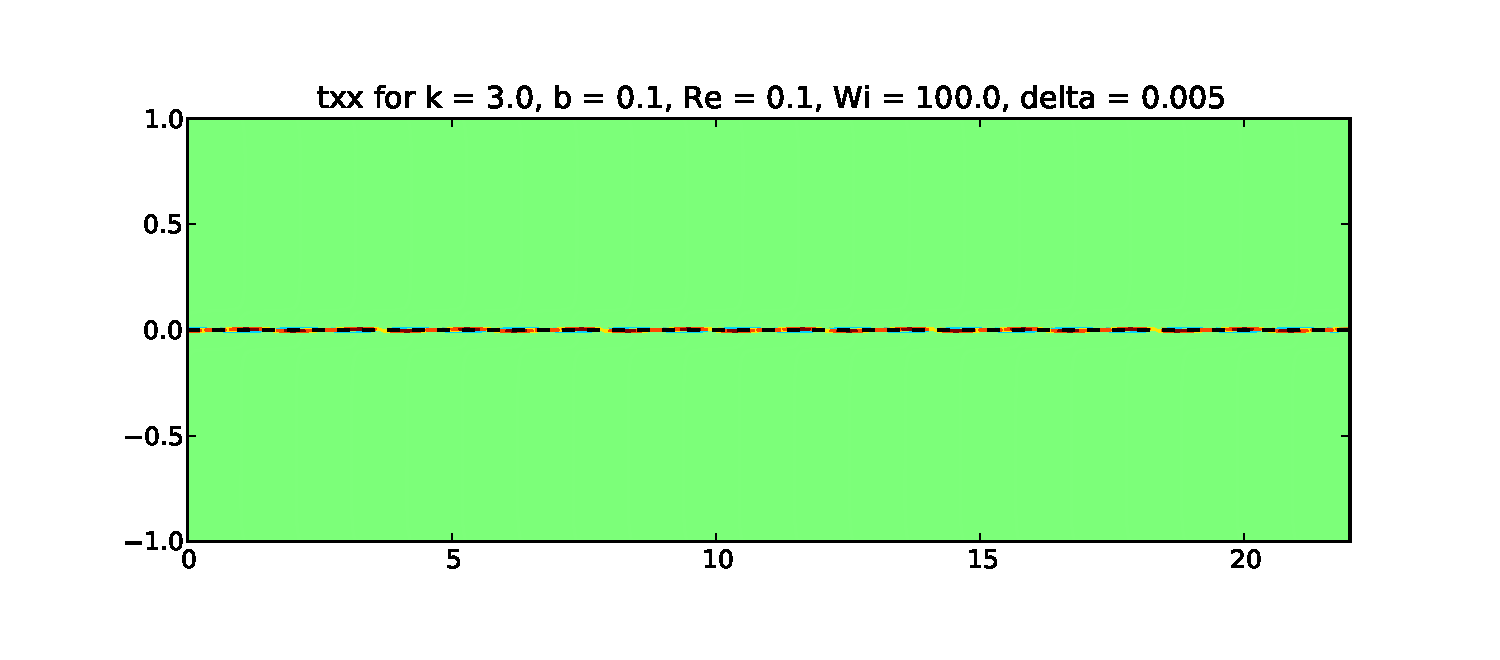
\includegraphics[width=\textwidth]{txx_low_delta} 
	\caption{}
	\label{fig:stress_low_delta} 
    \end{subfigure} 
    \caption{
	a) Streamfunction of the largest eigenfunction of the instability when
	$\Rey = 0.1$, $\Wi =100$, $\Delta = 0.005$. Red is positive
	(streamlines of the flow point clockwise around the contours), Blue is
	negative (streamlines of the flow point anticlockwise around the
	contours) b) xx stress for the same instability.  
    }
\end{figure}

Dependence of the instability on the channel walls persists at very small
$\Delta$ whilst in the purely elastic region of the flow phase space. We are
not sure why this is. We might be able to understand this by thinking about shear
waves in an elastic solid? (was thinking about surface Rayleigh waves)

\begin{figure} 
    \centering 
    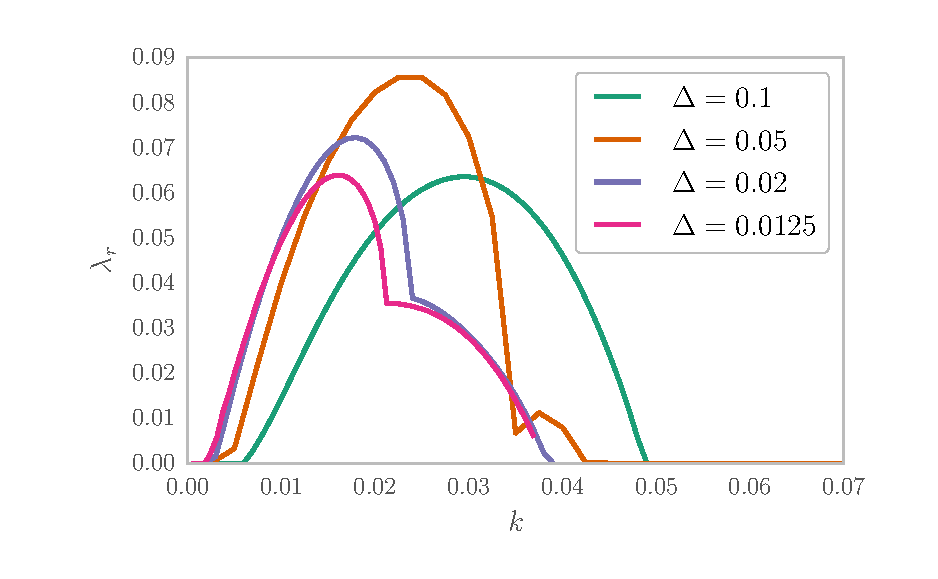
\includegraphics[width=\textwidth]{KH_vary_delta}
    \caption{
	Dispersion relations for various values of $\Delta$ at $\Rey = 0.1$,
	$\Wi = 100$. The sensitivity to the walls seems only to increase the
	strength of the instability. Even when the system is insensitive to the
	walls, at $\Delta= 0.0125$, there is still an instability present.
    } 
    \label{fig:walls_dependence} 
\end{figure}

\begin{figure} 
    \centering 
    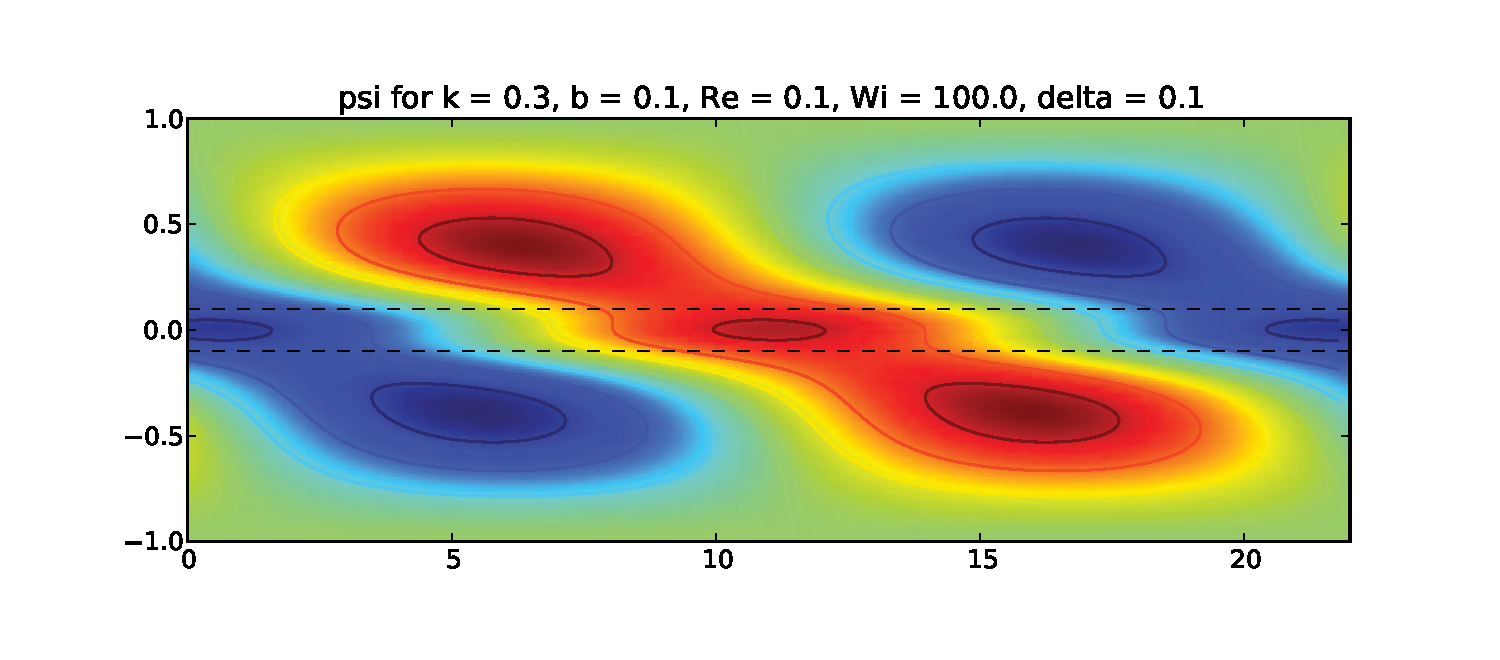
\includegraphics[width=\textwidth]{psi_high_delta}
    \caption{ 
	Streamfunction of the eigenfunction of the instability at $\Delta =
	0.1$, $\Wi = 100$, $\Rey=0.1$. The magnitude is scaled by the xx stress
	in the centre of the channel.  
    } 
    \label{fig:psi_high_delta}
\end{figure}

As the Reynold's number is reduced the walls become more important to the
instability, this makes a true $\Rey = 0$ instability difficult for us to
observe. In order to remove the dependence on the walls and recover a free
shear instability it is necessary to move them further away. This problem gets
worse at lower $\Rey$.  By introducing just a very small contribution from
inertia, we can remove the dependence on the walls. This is why all of our
results are taken for $\Rey \lesssim 0.1$ on the length scale of the
instability.

The reason we have have the simulation with the walls at all is because of the
implications for the plane Couette problem. The Kelvin-Helmholtz instability in
the Newtonian problem takes place on a length scale of about 10\% of the width
of the channel, or $\Delta = 0.1$. If this length scale is similar in the
purely elastic case, we can make say that the viscoelastic Kelvin-Helmholtz
instability is sensitive to the walls at this $\Delta$ and a $\Rey \lesssim 1$
(see figure \ref{fig:vary_Re_delta_conv}). This means that on the scale of the
channel, $\Rey \gtrsim 10$ for the walls not to affect the instability. So, the
important results for the purely elastic instability from the point of view of
the plane Couette problem are probably those for which the walls are relevant. 

\begin{figure} \centering
    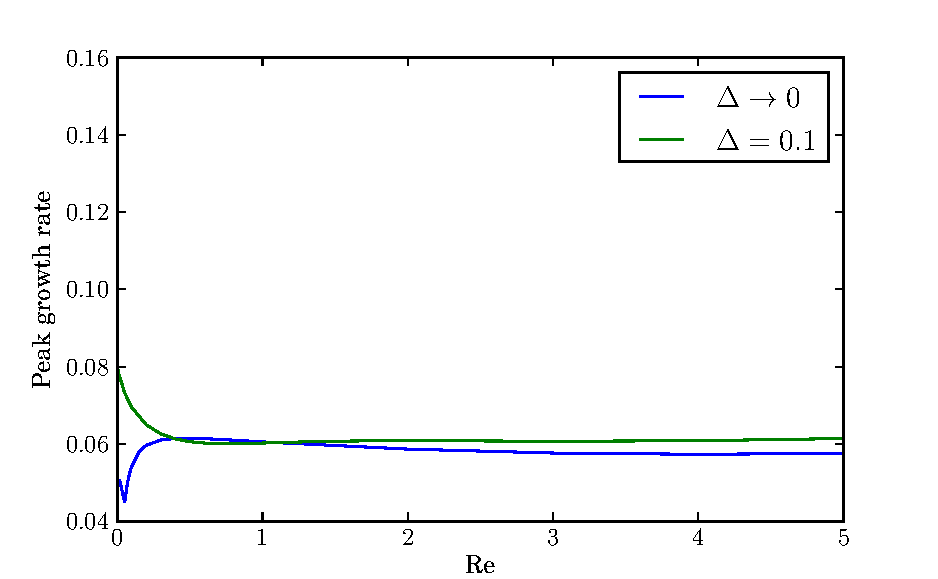
\includegraphics[width=0.7\textwidth]{vary_Re_delta_conv} \caption{ The
	blue line is the data from the free shear system and the green line is
	the $\Delta = 0.1$ data. By $\Rey = 1$ it is clear that the Reynold's
	number is sufficient such that the walled system behaves as though it
    were insensitive to the walls.  } \label{fig:vary_Re_delta_conv}
\end{figure}

At $\Delta = 0.1$ we see the same instability as that seen in the completely
free case. 

\begin{figure} 
    \centering 
    \begin{subfigure}[b]{0.48\textwidth} 
	\centering
	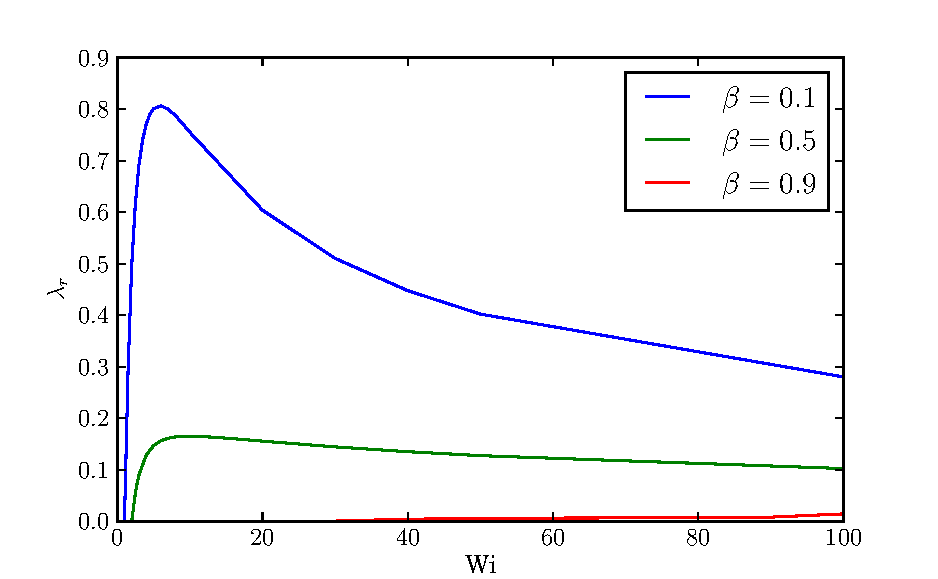
\includegraphics[width=\textwidth]{KH_low_Re_vary_Wi} 
	\caption{}
	\label{fig:KH_purely_elastic} 
    \end{subfigure} ~
    \begin{subfigure}[b]{0.48\textwidth} 
	\centering
	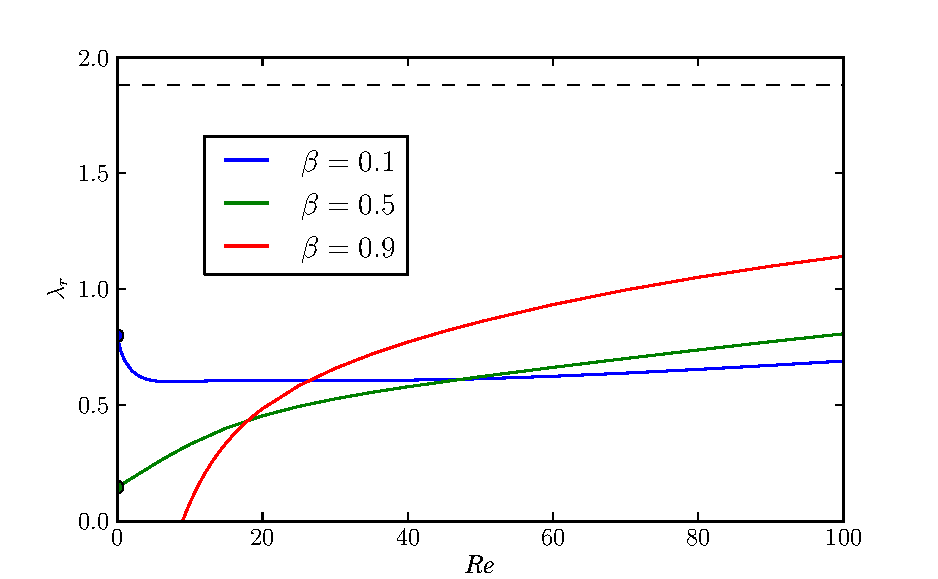
\includegraphics[width=\textwidth]{KH_low_Wi_vary_Re} 
	\caption{}
	\label{fig:KH_reduce_Re} 
    \end{subfigure}

    \begin{subfigure}[b]{0.48\textwidth} 
	\centering
	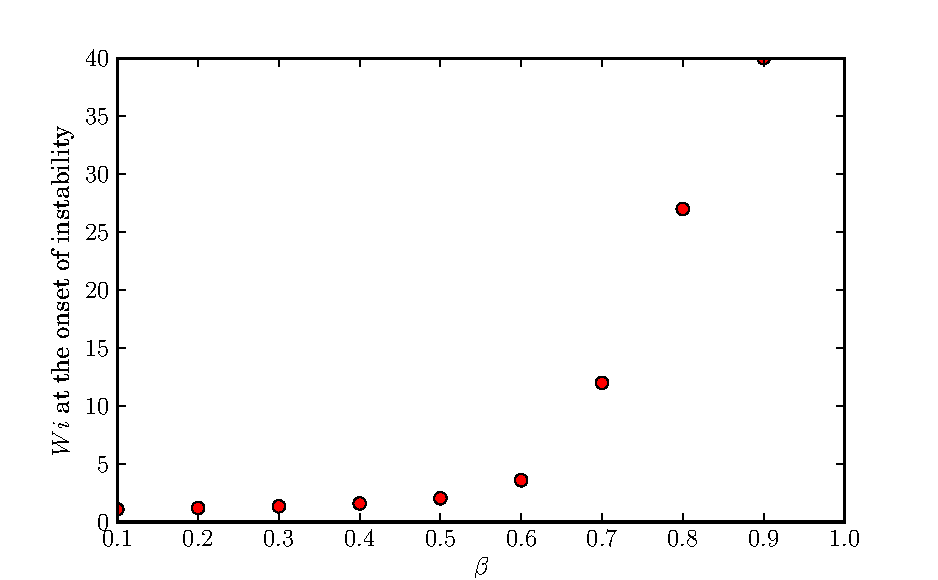
\includegraphics[width=\textwidth]{KH_onset_beta_Wi} 
	\caption{}
	\label{fig:KH_elastic_onset} 
    \end{subfigure} ~
    \begin{subfigure}[b]{0.48\textwidth} 
	\centering
	\includegraphics[width=\textwidth]{fin_dispersions_Wi50} 
	\caption{}
	\label{fig:KH_finite_dispersions} 
    \end{subfigure} 
    \caption{ 
	a) The change in the height of the dispersion relation as $\Wi$ is
	increased at $\Rey = 0$ with $\Delta = 0.1$. The green and red lines gives
	the behaviour at $\beta=0.1$, $\beta=0.5$ respectively. b) The change in
	the height of the dispersion relation as the Reynolds number is reduced at
	$\Wi=5.0$. The colours give the values of $\beta$ as above, with blue being
	the behaviour for $\beta=0.9$. At low $\Rey$ the instability is clearly
	still present for large polymer concentrations, consistent with purely
	elastic turbulence with $\Delta = 0.1$.  c) The value of the Weissenberg
	number at which the velocity profile becomes unstable against $\beta$ at
	$\Delta = 0.1$.  The onset of the purely elastic instability moves to
	higher $\Wi$ as $\beta$ increases. d) Dispersion relations at Wi =50 for
	$\Delta =0.1$.  
    }
\end{figure}


\begin{figure} 
    \centering
    \includegraphics[width=0.7\textwidth]{growth_rate_sldim} 
    \caption{ 
	Phase diagram showing the growth rate for various values of the
	Reynold's and Weissenberg numbers at $\beta=0.1$. Grey lines represent
	lines of constant elasticity. Black squares are data points for which
	the flow is linearly stable.  
    } 
    \label{fig:vary_Re_delta_conv} 
\end{figure}

\section{Confirming the model}

\subsection{Consistency of results with the FENE model}

The finite extensibility version of the model gives good agreement with the
Oldroyd-B version. Shorter lengths bring about a larger instability but do not
delay it to higher Weissenberg number. Otherwise similar dispersion relations
are observed with a similar dependence on the distance to the walls (figure
\ref{fig:FENE_low_Re}).

\begin{figure} 
    \centering
    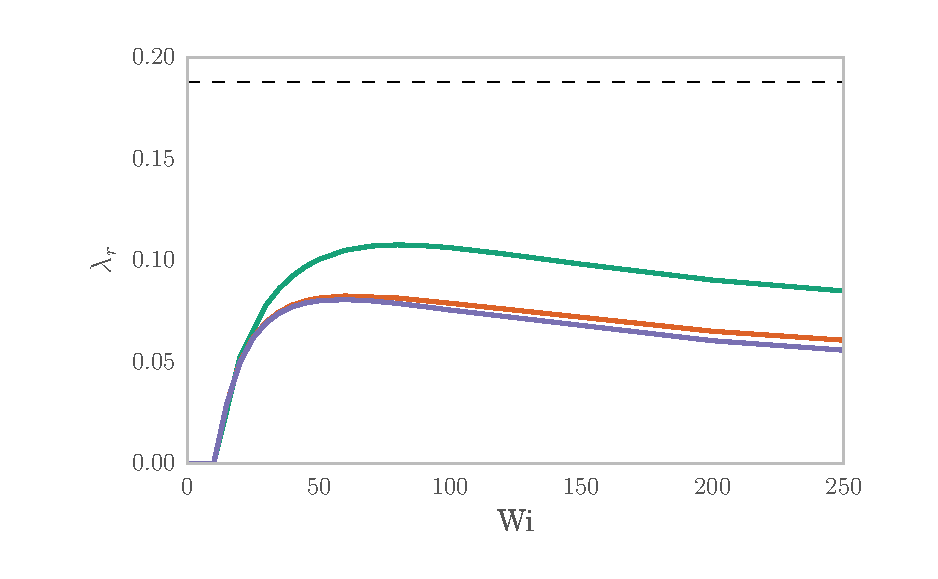
\includegraphics[width=0.7\textwidth]{FENE_purely_elastic} 
    \caption{ 
	The FENE-P model fluid at $\Rey = 0$  when $\Delta = 0.1$. Results are
	consistent with figure \ref{fig:KH_purely_elastic}.  
    }
	\label{fig:FENE_low_Re} \end{figure}

\subsection{Varying width of the instability}

\begin{figure} \centering
    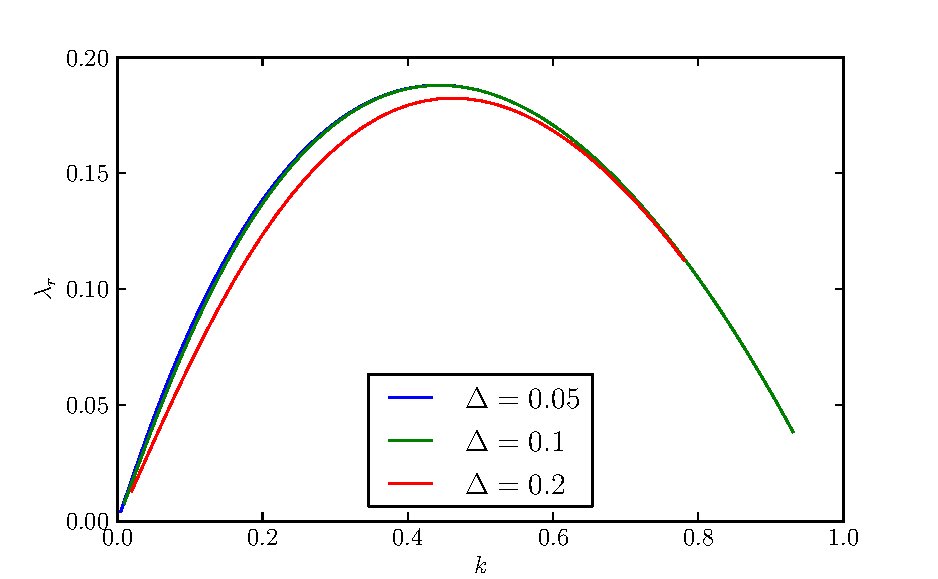
\includegraphics[width=0.7\textwidth]{high_Re_vary_delta} 
    \caption{
	Dispersion relations for various values of $\Delta$ and $\Rey = 1000$,
	$\Wi = 0.01$. When results are rescaled for delta, The instability is
	found to be insensitive to the width of the instability relative to the
	wall at this combination of Reynold's number and Weissenberg number.  
    }
    \label{fig:delta_dispersion}
\end{figure}


\subsection{Drag reduction}

We see drag reduction using the Oldroyd-B model. It is not clear whether or not
the maximum drag reduction asymptote is present (figure
\ref{fig:KH_drag_reduction}).

\begin{figure}
%   \showthe\columnwidth %use this to determine size of figures.
    \centering 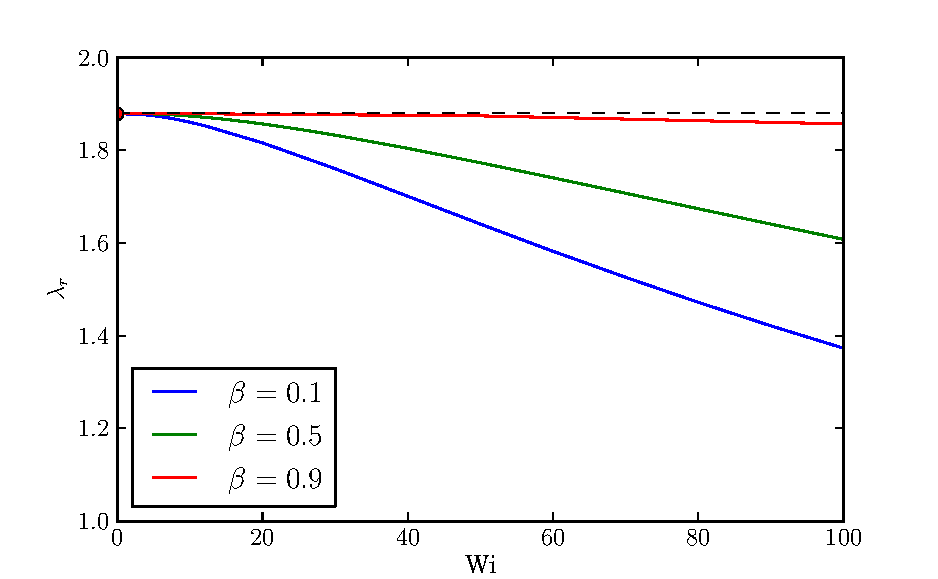
\includegraphics[width=0.7\textwidth]{KH_high_Re_vary_Wi}
    \caption{ 
	Peak growth rate against Weissenberg number at $\Rey = 1000$,
	$\Delta = 0.1$ The height of the dispersion relation is reduced for the
	Kelvin-Helmholtz instability as the Weissenberg number is increased.
	The grey dashed line is the height of the dispersion relation for the
	Newtonian fluid. The decrease in $\lambda_{r}$ corresponds to increased
	stability of the base flow and so confirms the presence of drag
	reduction in this system.  
    } 
    \label{fig:KH_drag_reduction} 
\end{figure}

\section{Conclusions}

In conclusion, we can say that there is a Kelvin-Helmholtz like instability for
purely elastic shear flows. The unstable region is much larger than that seen
in Newtonian fluids relative to the region of shear. The wavenumber of the
instability is much smaller in the viscoelastic case ($k<0.06$), suggesting a
larger minimal flow unit is required in viscoelastic fluids. This instability
is enhanced slightly by introducing a finite extensibility to the polymers but
remains of essentially the same form. The instability has grown to its maximum
by the time it reaches an effective Weissenberg number $ Wi \sim 50$ after
which it is saturated. The instability is also strongly dependent on the walls
at low Reynold's number.

\bibliographystyle{jfm}
%\bibliographystyle{plain}


\bibliography{KH_paper}

\end{document}
